

  % \begin{center}
  % 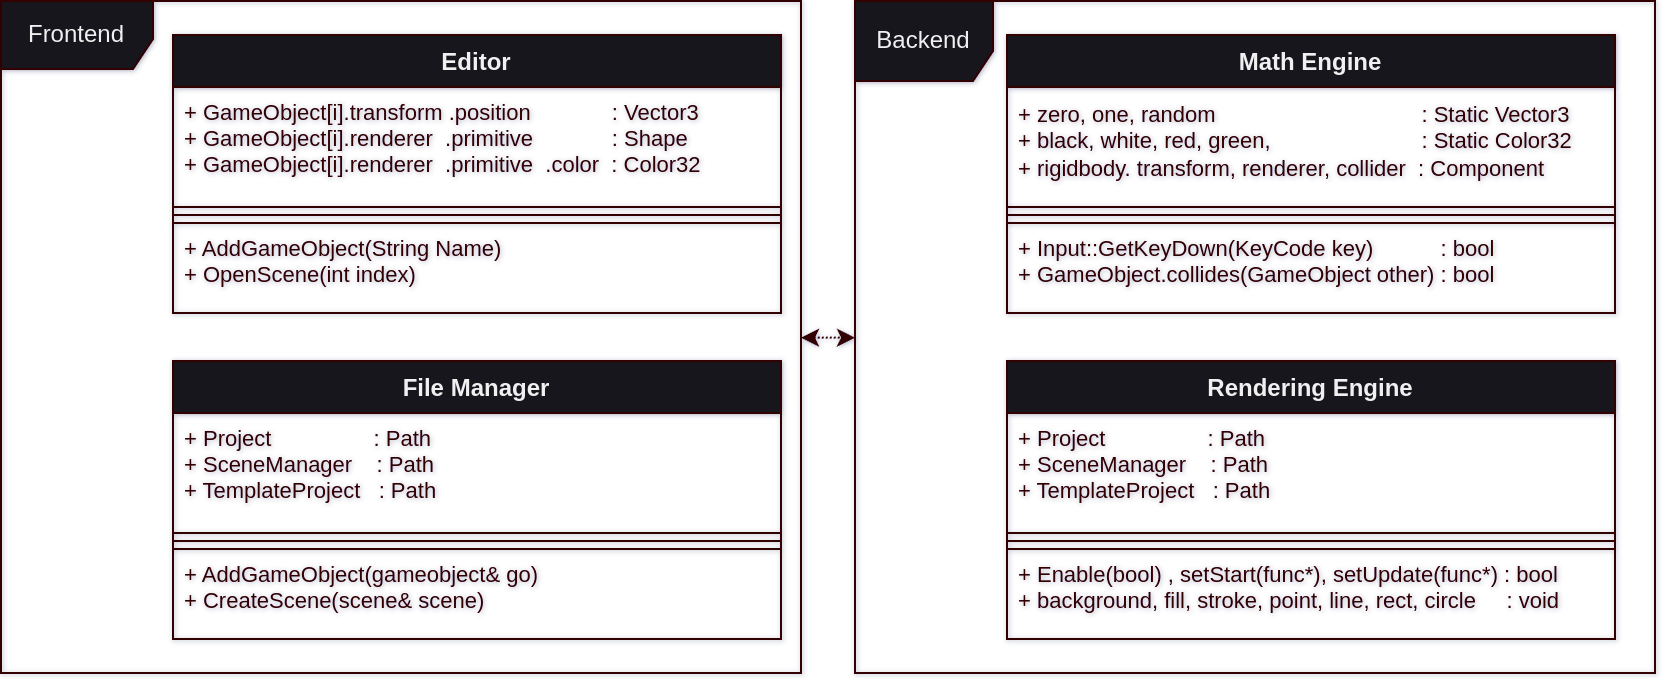
\includegraphics[width=1 \textwidth]{app_overview.png}
  % \end{center}





% \begin{center}
% 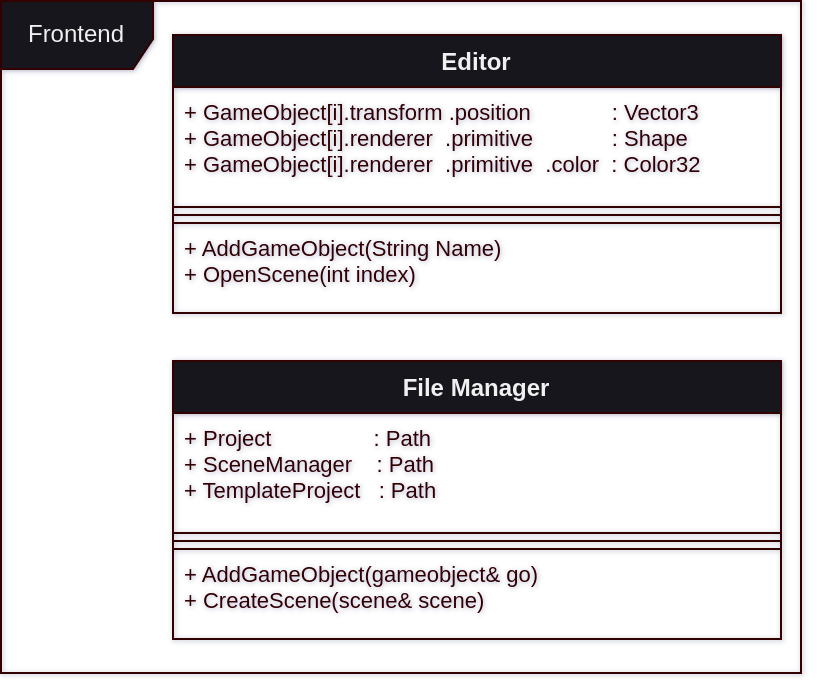
\includegraphics[width=0.486 \textwidth]{app_frontend_overview.png}
% \end{center}


% \begin{center}
% 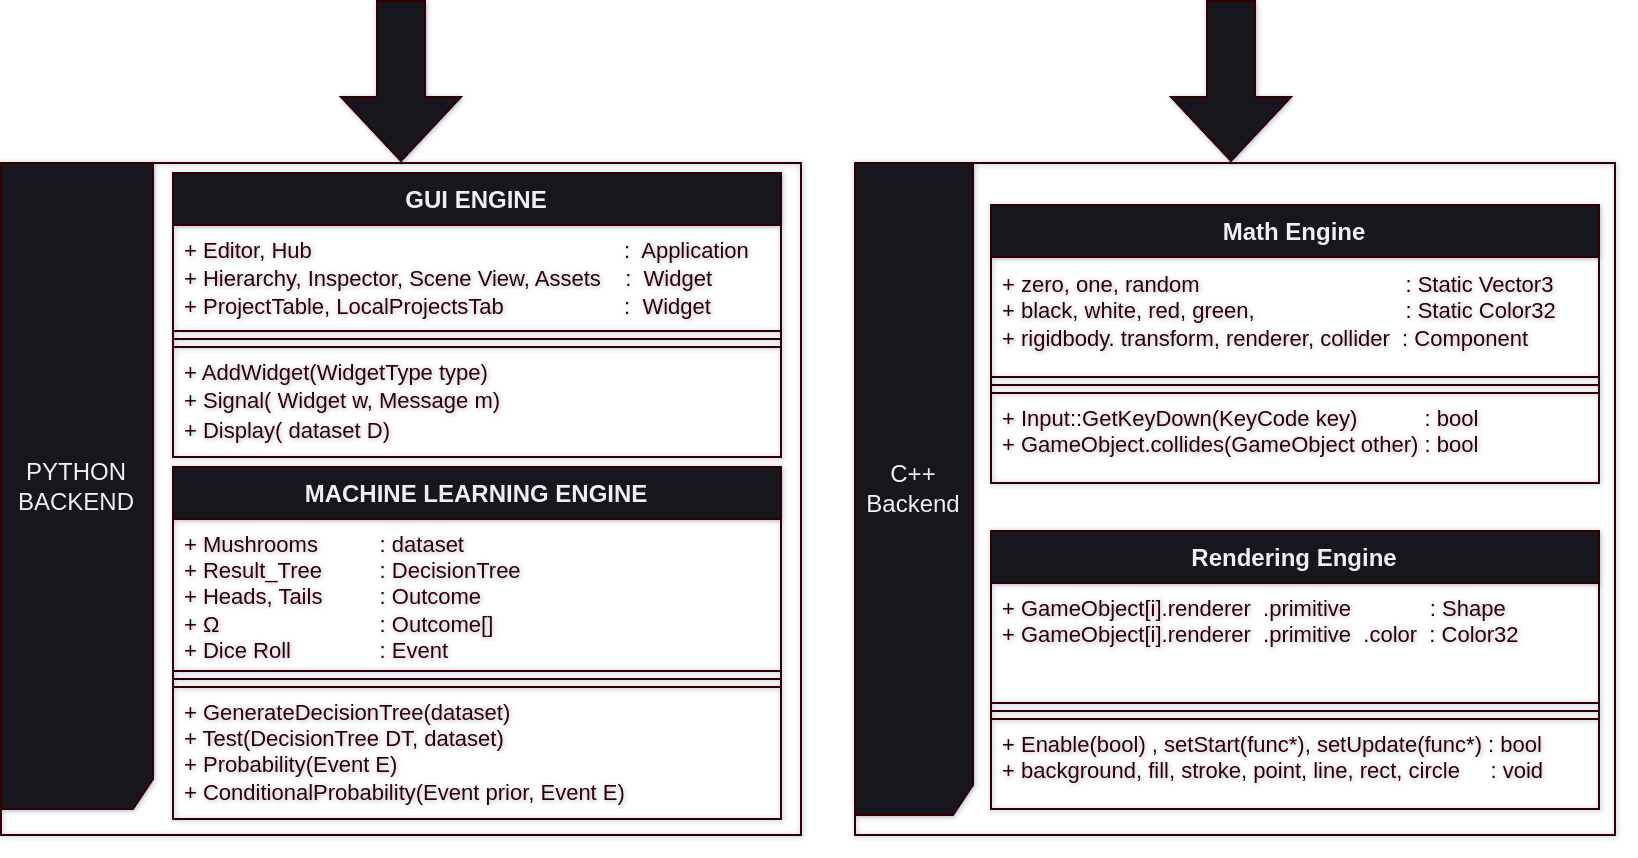
\includegraphics[width=0.9 \textwidth]{app_backend_overview.png}
% \end{center}




% \begin{minipage}[t]{0.45\textwidth}
%     \centering
%     \textbf{Frontend}
%     
%     \begin{tikzpicture}
%         \begin{axis}[
%             axis lines = left,
%             xlabel = $x$,
%             ylabel = {$y=f(x)$},
%         ]
%         \addplot [
%             domain=-10:10, 
%             samples=100, 
%             color=blue,
%         ]
%         {x^2};
%         \end{axis}
%     \end{tikzpicture}
% \end{minipage}
% \hfill
% \begin{minipage}[t]{0.45\textwidth}
%     \centering
%     \textbf{Backend}
%     
%     \begin{equation*}
%         \text{Input: } x = 3
%     \end{equation*}
%     \begin{equation*}
%         y = x^2 = 3^2 = 9
%     \end{equation*}
% \end{minipage}

% \vspace{0.5cm}

% \textbf{Interaction}

% \begin{minipage}[t]{0.3\textwidth}
%     \begin{equation*}
%         \text{Frontend: } \text{Enter } x
%     \end{equation*}
% \end{minipage}
% \begin{minipage}[t]{0.3\textwidth}
%     \begin{equation*}
%         \text{Backend: } y = x^2
%     \end{equation*}
% \end{minipage}
% \begin{minipage}[t]{0.3\textwidth}
%     \begin{equation*}
%         \text{Frontend: } y = 9
%     \end{equation*}
% \end{minipage}
